% Bash
\section{The Unix Shell}
You worked with a few Unix commands in the shell in the installation section. This section does a bit of a deeper dive into commands that you may find useful.

Being able to use the Unix Shell and terminal commands is an invaluable skill, and a requirement for this course. Follow \href{https://swcarpentry.github.io/shell-novice/}{this guide} (https://swcarpentry.github.io/shell-novice/) for more learning resources.

Some useful commands are listed below. There is also space to add your own commands if you find any that are useful.
\begin{table}[H]
\centering
\caption{Some useful shell commands}
\label{tbl:commands}
\begin{tabular}{|l|l|}
\hline
\textbf{Command} & \textbf{Use} \\ \hline
ls & \begin{tabular}[c]{@{}l@{}}List current files and folders in directory.\\ ls -al is useful to list everything\end{tabular} \\ \hline
pwd & Prints the current working directory  \\ \hline
cd \textless{}directory\textgreater{} & \begin{tabular}[c]{@{}l@{}}Change to a specified directory.\\ eg "cd .. " will take you one level up\end{tabular} \\ \hline
ifconfig & Shows details on current network interfaces\\ \hline
touch \textless{}file\textgreater{} & Create \textless{}file\textgreater{} \\ \hline
nano \textless{}file\textgreater{} & Opens \textless{}file\textgreater in the nano text editor \\ \hline
vim \textless{}file\textgreater{} & Opens \textless{}file\textgreater in the vim text editor \\ \hline
mkdir \textless{}dir\textgreater{} & Creates the folder specified in \textless{}dir\textgreater{} \\ \hline
sudo \textless{}cmd\textgreater{} & executes the command \textless{}cmd\textgreater with sudo privileges \\ \hline
raspi-config &  \begin{tabular}[c]{@{}l@{}}Must be run as administrator\\ Opens up the Raspberry Pi Configuration Tool\end{tabular} \\ \hline
man \textless{}command\textgreater{} & Opens the manual for a particular command \\ \hline
ssh & Creates an SSH session. See Section \ref{sec:SSH} \\ \hline
scp & Secure copy. See Section \ref{sec:SCP} \\ \hline
&  \\ \hline
&  \\ \hline
&  \\ \hline
&  \\ \hline
&  \\ \hline
\end{tabular}
\end{table}

\begin{figure}[H]
\centering
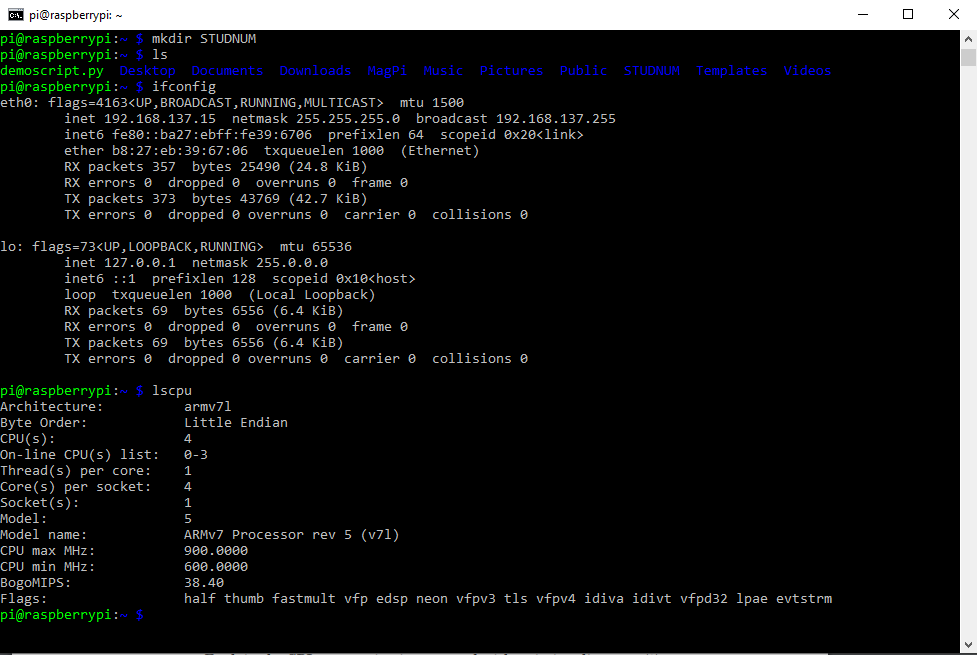
\includegraphics[width=1\columnwidth]{Figures/CMDOutput}
\caption{An example output of running some commands in the shell}
\end{figure}